\documentclass{article}

\usepackage[czech]{babel}
\usepackage[utf8]{inputenc}
\usepackage{fancyhdr}
\usepackage{amsmath}
\usepackage{amssymb}
\usepackage{hyperref}
\usepackage{url}
\usepackage{multirow}
\usepackage{array}
\usepackage{graphicx}
\usepackage{pdfpages}
\usepackage[margin=1.3in]{geometry}
\graphicspath{{./}}



\pagestyle{fancy}
\lhead{\small (II) Studium harmonických kmitů mechanického oscilátoru}
\rhead{\small Vladislav Wohlrath}

\begin{document}
\begin{titlepage}
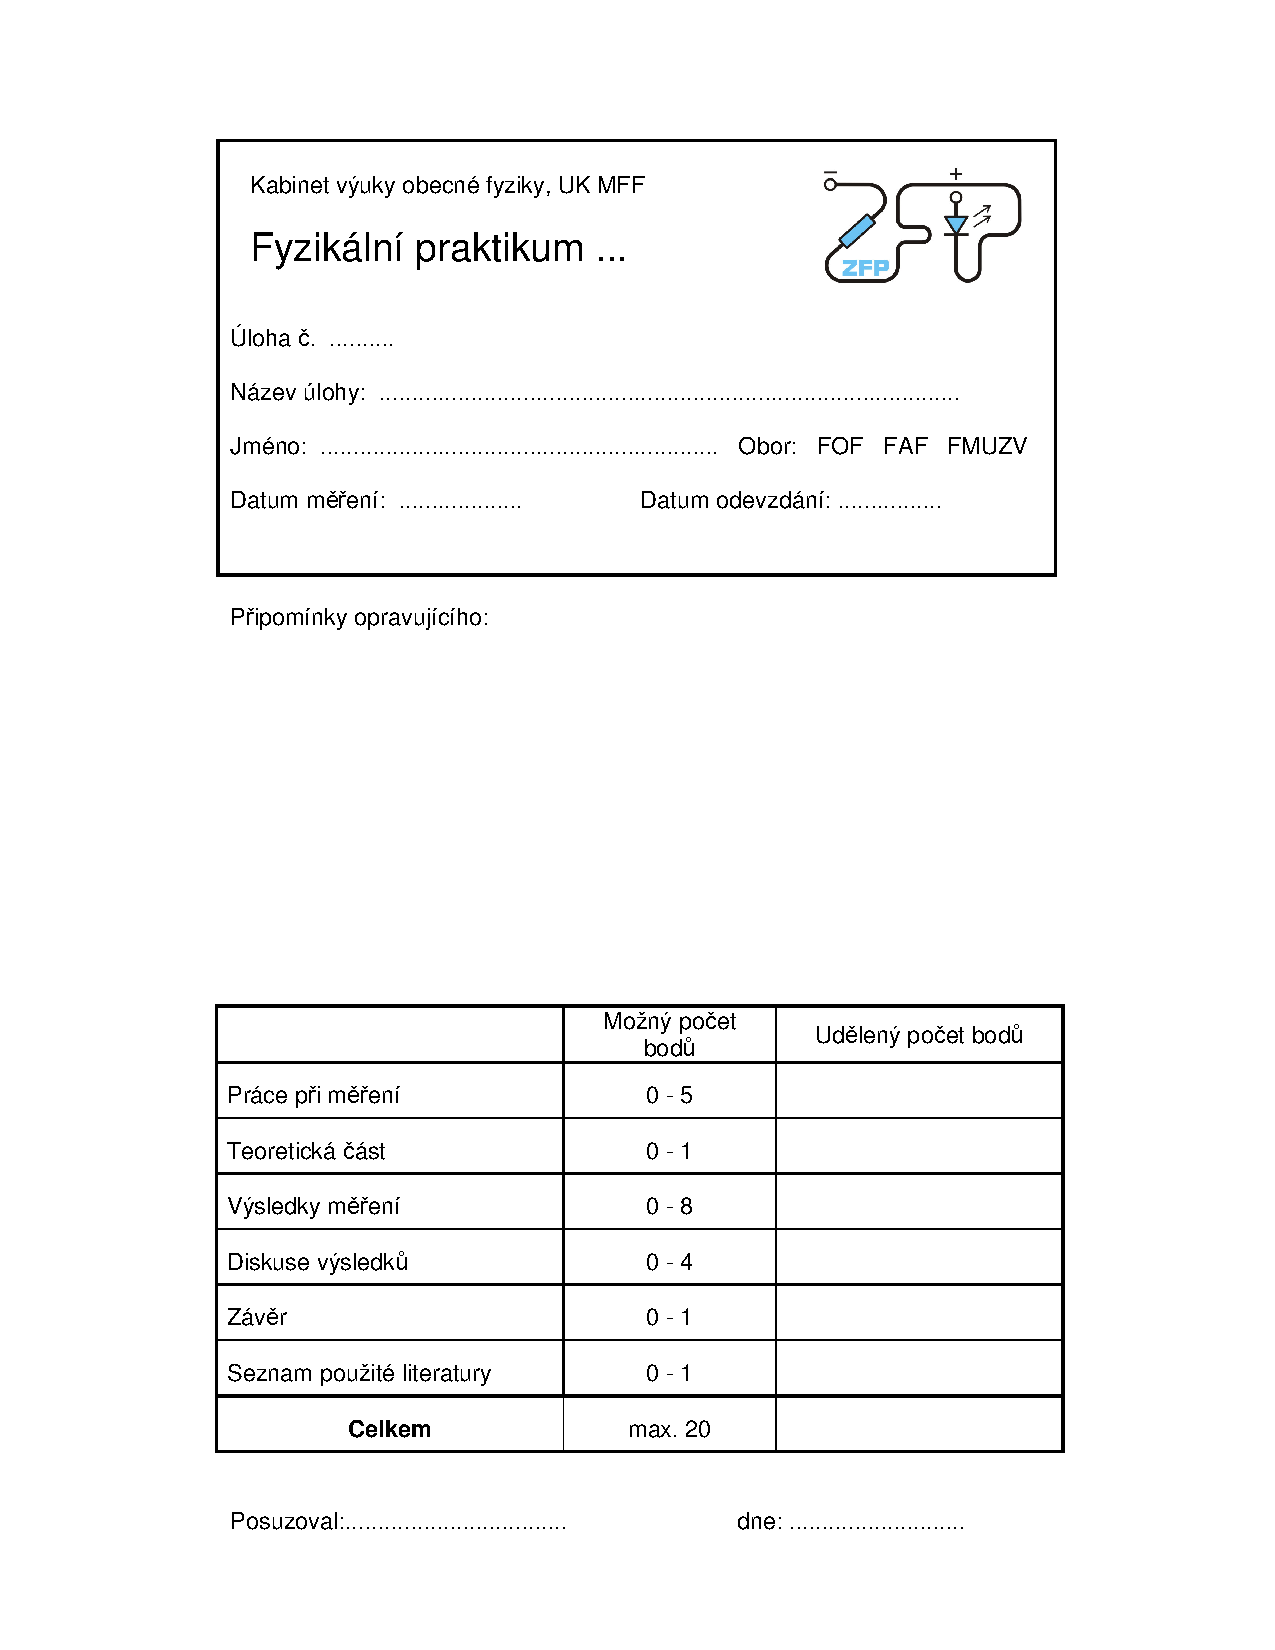
\includepdf[pages={1}]{titulka.pdf}

\end{titlepage}



\section*{Pracovní úkoly}
\begin{enumerate}
\item Změřte tuhost k pěti pružin metodou statickou.
\item Sestrojte graf závislosti prodloužení pružiny na působící síle $y=y(F)$.
\item Změřte tuhost k pěti pružin metodou dynamickou.
\item Z doby kmitu tělesa známé hmotnosti a výchylky pružiny po zavěšení tohoto tělesa určete místní tíhové zrychlení \emph{g}.
\item Sestrojte grafy závislostí:
\begin{description}
\item[a.] $\omega = f(\sqrt{k})$
\item[b.] $\omega = f(\sqrt{\frac{1}{m}})$
\end{description}
\item Při zpracování použijte lineární regresi.
\end{enumerate}

\section*{Teoretická část}

Síla $F_{D}$ potřebná k deformaci pružiny je přímo úměrná prodloužení pružiny $y$. 
\begin{equation} \label{eFD}
F_{D}=k \cdot y~.
\end{equation} 
Konstanta $k$ se nazývá tuhost pružiny.
\subsection*{Statická metoda}
Tuhost konkrétní pružiny lze snadno změřit statickou metodou \cite{ZFP}, při které pružinu deformujeme známou silou a měříme její prodloužení. V samotném experimentu budeme měřit závislost prodloužení $y_{0}$ na hmotnosti zavěšeného závaží $m$ a očekáváme lineární závislost
\begin{equation} \label{ey0}
y_{0}=a \cdot m~.
\end{equation}
Tuhost pružiny určíme z konstanty úměrnosti $a$ podle vztahu
\begin{equation} \label{ek}
k=\frac{g}{a}~,
\end{equation}
kde $g$ je tíhové zrychlení. Prodloužení pružiny měříme katetometrem, vzhledem k otřesům v laboratoři odhadujeme standardní odchylku $\sigma _{y0} = 2~mm$. Chyba hmotnosti závaží je vzhledem k chybě prodloužení zanedbatelná. Používáme tíhové zrychlení v~Praze $g=9,81373~ms^{-2}$ \cite{wolfram}.


Závislost $y_{0}=y_{0}(F)$ vyneseme do grafu jako
\begin{equation} \label{eyF}
y_{0}=\frac{a}{g} \cdot mg=\frac{a}{g} \cdot F~.
\end{equation}



\subsection*{Dynamická metoda}

Na závaží zavěšené na pružině působí síla směřující do rovnovážné polohy, jejíž velikost je přímo úměrná výchylce. Po vychýlení tedy vykonává harmonický pohyb daný funkcí
\begin{equation*}
y(t)=A \cdot sin(\omega t+ \phi)~,
\end{equation*}
kde $A$ je amplituda výchylky, $\phi$ je počáteční fáze, $\omega$ je úhlová rychlost a $t$ je čas. Úhlová rychlost je dána vztahem
\begin{equation} \label{eome}
\frac{2\pi}{T}= \omega = \sqrt{\frac{k}{m}}~.
\end{equation}


Tuhost pružiny můžeme měřit také dynamickou metodou \cite{ZFP}. Na pružinu zavěsíme závaží o hmotnosti $m$ a změříme dobu jednoho kmitu. Změříme závislost

\begin{equation}
\omega = b \cdot \frac{1}{\sqrt{m}}~.
\end{equation}
Z konstanty $b$ vypočteme tuhost pružiny jako
\begin{equation} \label{ekb}
k=b^{2}~.
\end{equation}


Měření provedeme elektronickým sonarem a pro větší přesnost měříme více kmitů. Standardní chybu měření odhadujeme na $0,1~s$.

\subsection*{Tíhové zrychlení}

Pokud změříme dvojici pružina-závaží statickou i dynamickou metodou, můžeme do (\ref{ey0}) a (\ref{ek}) dosadit známou tuhost a dostaneme tíhové zrychlení
\begin{equation} \label{etiha}
g=\omega ^{2}y_{0}~.
\end{equation}

\section*{Výsledky měření}

Měřili jsme celkem 5 pružin, označili jsme je písmeny A--E. Hmotnosti pružin a jejich délky v nenapjatém stavu jsou uvedeny v tabulce \ref{tpruziny}.


\begin{table}[htbp]
\begin{center}

\begin{tabular}{|c|c|c|}
\hline
pružina & \multicolumn{1}{l|}{délka (cm)} & \multicolumn{1}{l|}{hmotnost (g)} \\ \hline
A & 9,5 & 3,9 \\ \hline
B & 9,8 & 6,3 \\ \hline
C & 15,2 & 43,7 \\ \hline
D & 13,1 & 5,4 \\ \hline
E & 11,5 & 2,4 \\ \hline
\end{tabular}
\caption{Vlastnostni pružin}
\label{tpruziny}

\end{center}
\end{table}

\subsection*{Statická metoda}
Pro každou pružinu jsme změřili prodloužení pro 5 až 6 různých zatížení. Střední hodnotu konstanty $a$ v rovnici (\ref{ey0}) určíme pomocí vztahu (\ref{eenglich}) \cite{englich}

\begin{equation} \label{eenglich}
\tilde a = \frac{\sum_{i=1}^{n} m_{i}^{2}}{\sum_{i=1}^{n} m_{i}y_{0i}}~,
\end{equation}



\begin{table}[htbp]
\begin{center}
\begin{tabular}{|c||r|r|r|r|r|}
\hline
pružina & $m_{i} (g)$ & $y_{0i} (mm)$ & $m_{i} y_{0i} (g \cdot mm)$ & $m_{i}^{2} (g^{2})$ & $k_{i} (N \cdot m^{-1})$\\ [0.5ex]

\hline \hline
\multirow{6}{*}{\centering A} & 100 & 33 & 3300 & 10000 & 29,7 \\
& 120 & 39 & 4680 & 14400 & 30,2 \\ 
& 150 & 49 & 7350 & 22500  & 30,0\\ 
& 250 & 81 & 20250 & 62500  & 30,3\\ 
& 370 & 121 & 44770 & 136900 & 30,0\\ 
& 500 & 163 & 81500 & 250000  & 30,1\\ \hline
\multirow{6}{*}{\centering B} & 20 & 27 & 540 & 400 & 7,3\\ 
 & 50 & 66 & 3300 & 2500 & 7,4\\
 & 100 & 135 & 13500 & 10000 & 7,3\\ 
 & 120 & 161 & 19320 & 14400 & 7,3\\ 
 & 150 & 201 & 30150 & 22500 & 7,3\\ 
 & 200 & 267 & 53400 & 40000 & 7,3\\ \hline
\multirow{5}{*}{\centering C} & 100 & 17 & 1700 & 10000 & 57,7 \\
 & 120 & 21 & 2520 & 14400 & 56,1\\ 
 & 150 & 29 & 4350 & 22500 & 50,7\\ 
 & 250 & 61 & 15250 & 62500 & 40,2\\ 
 & 500 & 146 & 73000 & 250000 & 33,6\\ \hline
\multirow{5}{*}{\centering D} & 20 & 57 & 1140 & 400 & 3,4\\
 & 50 & 144 & 7200 & 2500 & 3,4\\ 
 & 100 & 287 & 28700 & 10000 & 3,4\\ 
 & 120 & 344 & 41280 & 14400 & 3,4\\ 
 & 150 & 429 & 64350 & 22500 & 3,4\\ \hline
\multirow{5}{*}{\centering E} & 50 & 31 & 1550 & 2500 & 15,8\\
 & 100 & 64 & 6400 & 10000 & 15,3\\
 & 120 & 77 & 9240 & 14400 & 15,3\\
 & 150 & 98 & 14700 & 22500 & 15,0\\
 & 250 & 162 & 40500 & 62500 & 15,1\\ \hline
\end{tabular}
\caption{Statická metoda: naměřené hodnoty}
\label{tstatikadata}

\end{center}

\end{table}

Naměřené hodnoty jsou uvedeny v tabulce \ref{tstatikadata}. V posledním sloupci jsou uvedeny tuhosti pro každé měření. Je zřejmé, že pružina C není lineární v celé oblasti měření. Hodnoty pro dvě nejmenší zatížení nebudeme dále zpracovávat a tuhost určíme podle zbylých tří. Dále spočítáme disperzi podle vztahu (\ref{edisperze}) \cite{englich}


\begin{equation} \label{edisperze}
D_{\tilde{a}}=\frac{\sigma _{y_{0}}^{2}}{\sum_{i=1}^{n} m_{i}^{2}}~,
\end{equation}
kde $\sigma_{y_{0}} = 2~mm$ je chyba měření prodloužení. Po odmocnění disperze a použití vztahu (\ref{ek}) dostáváme pro jednotlivé pružiny hodnoty v tabulce \ref{ttuhosti} (P=0,68). Chybu tuhosti počítáme podle vztahu (\ref{echybak}). Závislost (\ref{eyF}) je vynesena do grafu (obr. 1).

\begin{equation} \label{echybak}
\sigma _{\tilde{k}}^{2}=   (\frac{\partial k}   {\partial a})^{2} \cdot \sigma _{\tilde{a}}^{2} = \frac{\tilde{k} ^{2}}{\tilde{a}^{2}} \cdot \sigma _{\tilde{a}}^{2}
\end{equation}

\begin{table}[htbp]
\begin{center}
\begin{tabular}{|c|r|r|r|r|}
\hline
pružina & 
\multicolumn{1}{c|}{$\tilde{a} (m \cdot kg^{-1})$} & 
\multicolumn{1}{c|}{$\sigma _{\tilde{a}} (m \cdot kg^{-1})$} & 
\multicolumn{1}{c|}{$\tilde{k} (N \cdot m^{-1})$} & 
\multicolumn{1}{c|}{$\sigma _{\tilde{k}} (N \cdot m^{-1})$} \\ \hline
A & 0,326 & 0,0028 & 30,093 & 0,262 \\ \hline
B & 1,339 & 0,0067 & 7,331 & 0,037 \\ \hline
C & 0,276 & 0,0035 & 35,503 & 0,444 \\ \hline
D & 2,865 & 0,0090 & 3,426 & 0,011 \\ \hline
E & 0,647 & 0,0060 & 15,170 & 0,140 \\ \hline
\end{tabular}
\caption{Statická metoda: výsledky}
\label{ttuhosti}
\end{center}
\end{table}


\begin{figure} \label{gyf} 
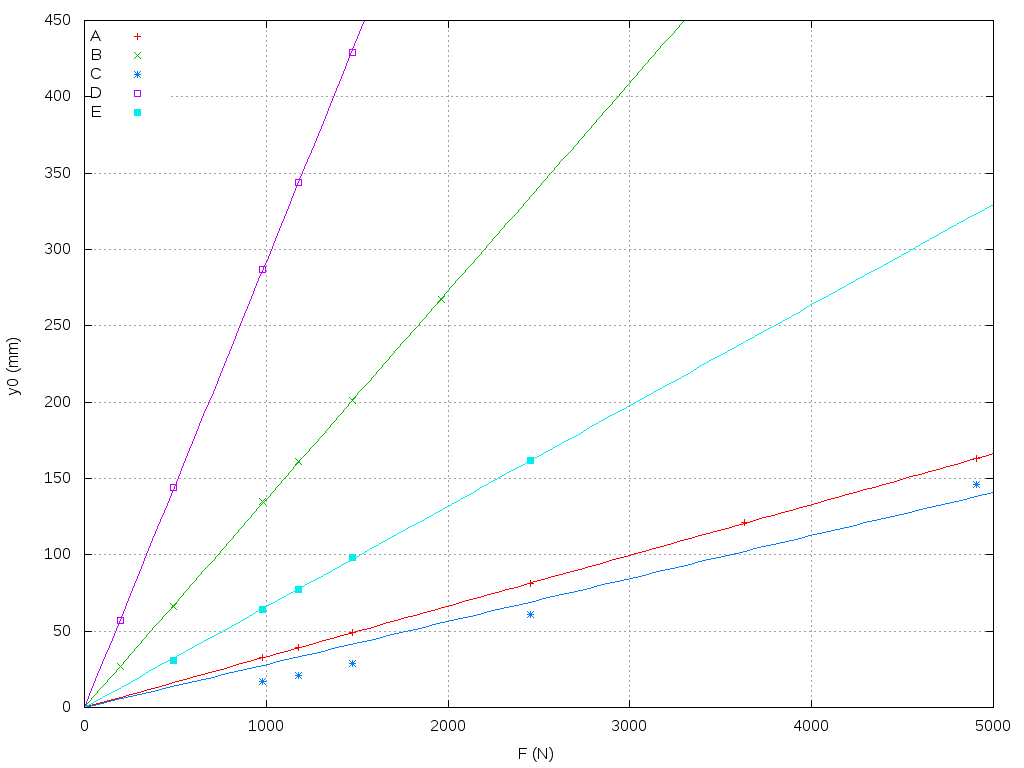
\includegraphics[width=\textwidth]{gyf}

\caption{Graf závislosti prodloužení na tíhové síle závaží}
\end{figure} 

\subsection*{Dynamická metoda}

Pro každou pružinu jsme měřili periodu při stejném zatížení jako při statické metodě. Naměřené hodnoty jsou uvedeny v tabulce \ref{tdyndata}. Vypočteme veličinu $1/\sqrt{m}$, z doby kmitu podle vztahu (\ref{eome}) úhlovou rychlost $\omega$ a její chybu podle
\begin{equation*}
\sigma _{\tilde{\omega}}^{2}=   (\frac{\partial \omega}   {\partial T})^{2} \cdot \sigma _{\tilde{T}}^{2} = \frac{\tilde{\omega} ^{2}}{\tilde{T}^{2}} \cdot \sigma _{\tilde{T}}^{2}
\end{equation*}

Chybu jednoho kmitu bereme jako chybu měření $0,1s$ dělenou počtem měřených kmitů.


\begin{table}[htbp]
\begin{center}
\begin{tabular}{|c||r|r|r|r|r|r|}
\hline
\multicolumn{1}{|c||}{pružina} & \multicolumn{1}{c|}{$m_{i} (g)$} & \multicolumn{1}{c|}{$1/\sqrt{m_{i}} ~(kg^{-1/2})$} & \multicolumn{1}{c|}{$T_{i} ~(s)$} & \multicolumn{1}{c|}{$\sigma _{Ti} ~(s)$} & \multicolumn{1}{c|}{$\omega _{i} ~(s^{-1})$} & \multicolumn{1}{c|}{$\sigma _{\omega i} ~(s^{-1}) $} \\ \hline \hline
\multirow{6}{*}{\centering A} & 100 & 3,162 & 0,368 & 0,00588 & 17,09 & 0,273 \\ 
&  120 & 2,887 & 0,400 & 0,00714 & 15,71 & 0,280 \\ 
&  150 & 2,582 & 0,445 & 0,00625 & 14,12 & 0,198 \\ 
 & 250 & 2,000 & 0,571 & 0,00667 & 11,01 & 0,129 \\ 
&  370 & 1,644 & 0,695 & 0,00455 & 9,05 & 0,059 \\ 
&  500 & 1,414 & 0,804 & 0,00357 & 7,81 & 0,035 \\ \hline
\multirow{6}{*}{\centering B} & 20 & 7,071 & 0,346 & 0,00270 & 18,16 & 0,142 \\ 
&  50 & 4,472 & 0,531 & 0,00455 & 11,83 & 0,101 \\ 
&  100 & 3,162 & 0,741 & 0,00588 & 8,48 & 0,067 \\ 
&  120 & 2,887 & 0,811 & 0,00526 & 7,75 & 0,050 \\
&  150 & 2,582 & 0,903 & 0,00625 & 6,96 & 0,048 \\ 
&  200 & 2,236 & 1,038 & 0,00526 & 6,05 & 0,031 \\ \hline
\multirow{5}{*}{\centering C} & 100 & 3,162 & 0,331 & 0,00345 & 18,98 & 0,198 \\ 
&  120 & 2,887 & 0,379 & 0,00357 & 16,60 & 0,157 \\
&  150 & 2,582 & 0,431 & 0,00435 & 14,57 & 0,147 \\ 
&  250 & 2,000 & 0,596 & 0,00476 & 10,54 & 0,084 \\ 
&  500 & 1,414 & 0,845 & 0,00435 & 7,43 & 0,038 \\ \hline
\multirow{5}{*}{\centering D}  & 20 & 7,071 & 0,506 & 0,00238 & 12,42 & 0,058 \\ 
&  50 & 4,472 & 0,777 & 0,00357 & 8,08 & 0,037 \\ 
&  100 & 3,162 & 1,084 & 0,00476 & 5,80 & 0,025 \\
&  120 & 2,887 & 1,183 & 0,00526 & 5,31 & 0,024 \\ 
&  150 & 2,582 & 1,318 & 0,00588 & 4,77 & 0,021 \\ \hline
\multirow{5}{*}{\centering E}  & 50 & 4,472 & 0,366 & 0,00385 & 17,16 & 0,180 \\ 
&  100 & 3,162 & 0,514 & 0,00476 & 12,22 & 0,113 \\
&  120 & 2,887 & 0,562 & 0,00526 & 11,18 & 0,105 \\ 
&  150 & 2,582 & 0,629 & 0,00556 & 9,99 & 0,088 \\ \
&  250 & 2,000 & 0,806 & 0,00476 & 7,80 & 0,046 \\ \hline
\end{tabular}
\caption{Dynamická metoda: naměřené hodnoty}
\label{tdyndata}
\end{center}

\end{table}



Střední hodnotu veličiny $b$ vypočítáme podle vztahu (\ref{eb}) \cite{englich}

\begin{equation} \label{eb}
\tilde{b} = \frac    {\sum_{i=1}^{n}  \frac{\omega _{i}}{  \sqrt{m_{i}} \sigma _{\omega i}^{2   }  }  }      {\sum_{i=1}^{n}  \frac   {1}         {m_{i} \sigma _{\omega i}^{2}     }}
\end{equation}
a její disperzi podle \cite{englich}

\begin{equation*}
D_{\tilde{b}} = \frac{1}{\sum_{i=1}^{n}  \frac{1}  {m_{i} \sigma _{\omega i} ^{2}    }                     }~.
\end{equation*} 

Tuhost pružiny získáme z $b$ díky vztahu (\ref{ekb}) a její chybu jako
\begin{equation*}
\sigma _{\tilde{k}}^{2}=   (\frac{\partial k}   {\partial b})^{2} \cdot \sigma _{\tilde{b}}^{2} = \frac{4 \tilde{k} ^{2}}{\tilde{b}^{2}} \cdot \sigma _{\tilde{b}}^{2}
\end{equation*}

Výsledné hodnoty veličiny $b$, tuhosti a jejich výchylek jsou uvedeny v tabulce \ref{tdynvysl}. Grafy závislostí úhlové rychlosti na $\sqrt{k}$ a $\sqrt{1/m}$ jsou zaneseny do grafů (obr. 2) a (obr. 3) resp. (pozn.)

\begin{table}[htbp]
\begin{center}
\begin{tabular}{|c|r|r|r|r|}
\hline
pružina & \multicolumn{1}{c|}{$ \tilde{b} ~(kg^{1/2}s^{-1})    $} & \multicolumn{1}{c|}{$  \sigma _{\tilde{b}}   ~(kg^{1/2}s^{-1})   $}
 & \multicolumn{1}{c|}{$ \tilde{k}  ~(N \cdot m^{-1})           $}
  & \multicolumn{1}{c|}{$ \sigma _{\tilde{k}}  ~(N\cdot m^{-1})           $} \\ \hline
A & 5,51 & 0,0180 & 30,32 & 0,198 \\ \hline
B & 2,67 & 0,0074 & 7,14 & 0,040 \\ \hline
C & 5,43 & 0,0188 & 29,46 & 0,204 \\ \hline
D & 1,82 & 0,0037 & 3,30 & 0,013 \\ \hline
E & 3,88 & 0,0143 & 15,03 & 0,111 \\ \hline
\end{tabular}
\caption{Dynamická metoda: výsledky}
\label{tdynvysl}
\end{center}
\end{table}


\begin{figure} \label{gwk} 
\centering
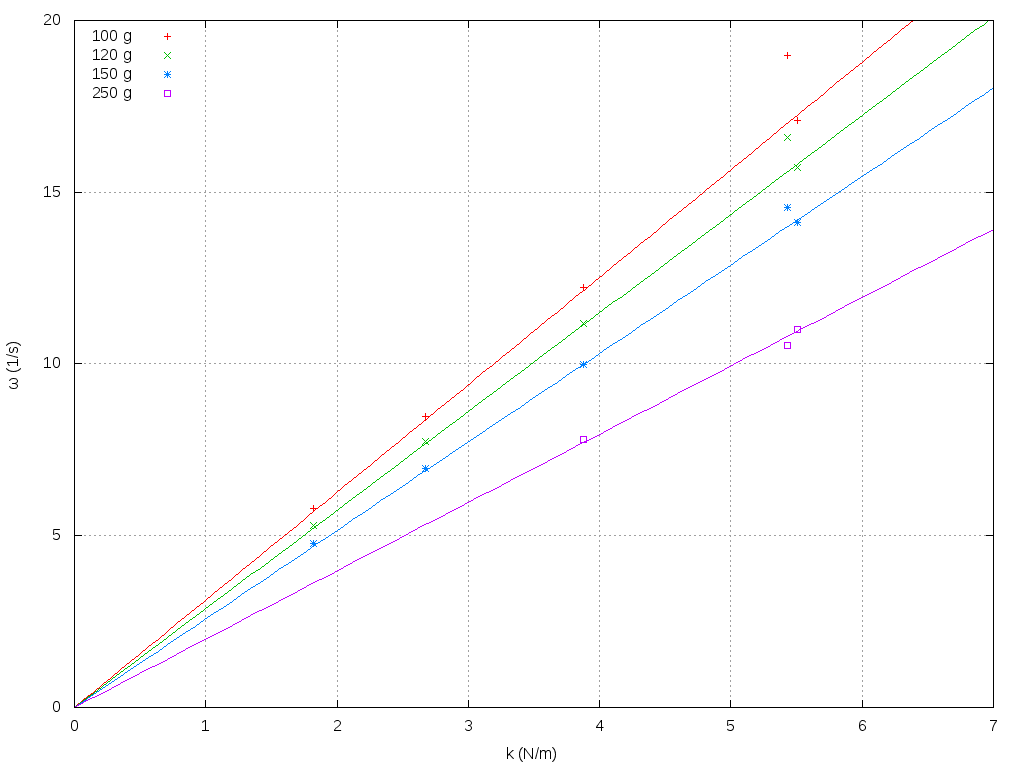
\includegraphics[width=\textwidth]{gwk}
\caption{Graf závislosti $ \omega = F(\sqrt{k}) $}
\end{figure} 


\begin{figure} \label{gwm} 
\centering
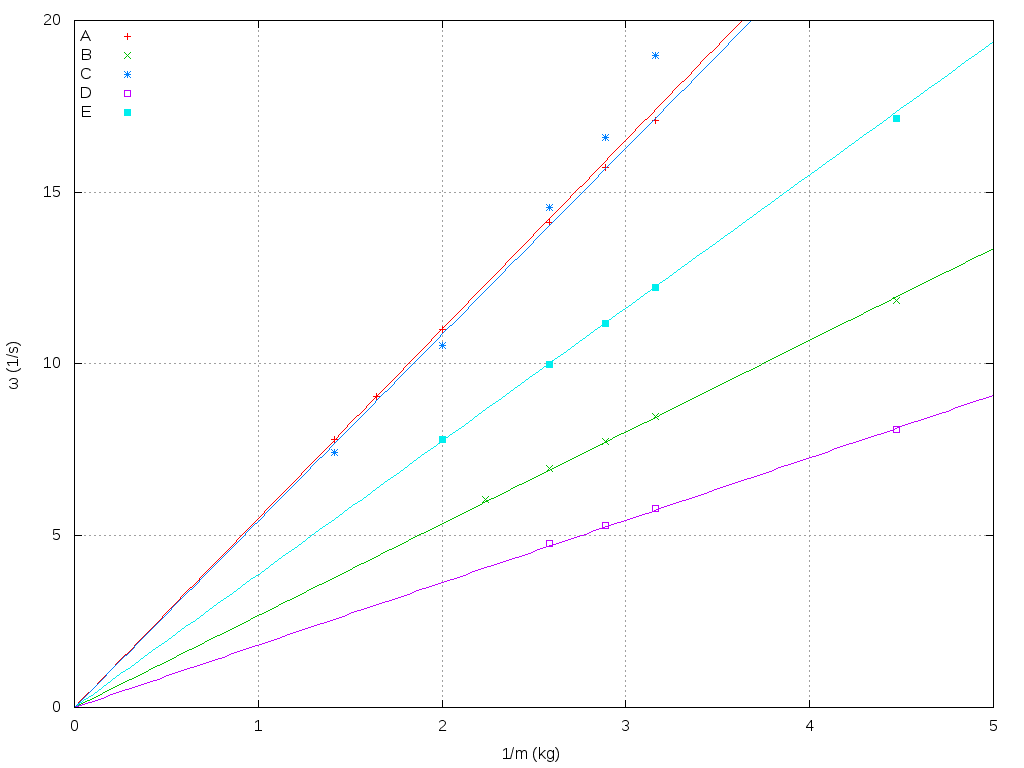
\includegraphics[width=\textwidth]{gwm}
\caption{Graf závislosti $ \omega = F(\sqrt{\frac{1}{m}}) $ (pozn.: přímka náležící pružině C je zdánlivě proložena špatně, mějmě ale na paměti, že jsou to právě hodnoty blízké počátku, které jsou nejpřesnější)}
\end{figure} 


\subsection*{Tíhové zrychlení}

Hodnoty tíhového zrychlení vypočtené z (\ref{etiha}) pro každé měření jsou uvedeny v tabulce \ref{ttiha}. Průměrné hodnoty a jejich standardní odchylky jsou uvedené v tabulce \ref{ttihavysl}.

\begin{table}[htbp]
\begin{center}
\begin{tabular}{|c||r|r|r|r|}
\hline
pružina & \multicolumn{1}{c|}{$m_{i} (g)$} & \multicolumn{1}{c|}{$y_{0i} (mm)$} & \multicolumn{1}{c|}{$\omega _{i} ~(s^{-1})$} & \multicolumn{1}{c|}{$ g ~(ms^{-2})   $} \\ \hline \hline
\multirow{6}{*}{A} & 100 & 33 & 17,09 & 9,64 \\ 
 & 120 & 39 & 15,71 & 9,62 \\ 
 & 150 & 49 & 14,12 & 9,77 \\ 
 & 250 & 81 & 11,01 & 9,82 \\ 
 & 370 & 121 & 9,05 & 9,90 \\ 
 & 500 & 163 & 7,81 & 9,95 \\ \hline
\multirow{6}{*}{B} & 20 & 27 & 18,16 & 8,91 \\
 & 50 & 66 & 11,83 & 9,24 \\
 & 100 & 135 & 8,48 & 9,70 \\
 & 120 & 161 & 7,75 & 9,68 \\ 
 & 150 & 201 & 6,96 & 9,74 \\ 
 & 200 & 267 & 6,05 & 9,79 \\ \hline
\multirow{5}{*}{C} & 100 & 17 & 18,98 & 6,12 \\
 & 120 & 21 & 16,60 & 5,78 \\
 & 150 & 29 & 14,57 & 6,15 \\ 
 & 250 & 61 & 10,54 & 6,78 \\ 
 & 500 & 146 & 7,43 & 8,07 \\ \hline
\multirow{5}{*}{D} & 20 & 57 & 12,42 & 8,80 \\ 
 & 50 & 144 & 8,08 & 9,41 \\
 & 100 & 287 & 5,80 & 9,65 \\ 
 & 120 & 344 & 5,31 & 9,70 \\
 & 150 & 429 & 4,77 & 9,75 \\ \hline
\multirow{5}{*}{E} & 50 & 31 & 17,16 & 9,13 \\ 
 & 100 & 64 & 12,22 & 9,55 \\ 
 & 120 & 77 & 11,18 & 9,62 \\ 
 & 150 & 98 & 9,99 & 9,78 \\ 
 & 250 & 162 & 7,80 & 9,85 \\ \hline
\end{tabular}
\caption{Hodnoty tíhového zrychlení pro jednotlivá měření}
\label{ttiha}
\end{center}

\end{table}

\begin{table}[htbp]
\begin{center}
\begin{tabular}{|c|r|r|}
\hline
pružina & \multicolumn{1}{c|}{$ g ~(ms^{-2})   $} & \multicolumn{1}{c|}{$ \sigma _{g} ~(ms^{-2})   $} \\ \hline
A & 9,78 & 0,13 \\ \hline
B & 9,51 & 0,35 \\ \hline
C & 6,58 & 0,90 \\ \hline
D & 9,46 & 0,39 \\ \hline
E & 9,59 & 0,28 \\ \hline
\end{tabular}
\caption{Tíhové zrychlení}
\label{ttihavysl}
\end{center}

\end{table}




\section*{Diskuze výsledků}

Výsledky v tabulce \ref{ttiha} a \ref{ttihavysl} můžeme využít ke kontrole, tíhové zrychlení by mělo být přibližně $9,8~ms^{-2}$. Z výsledků je zřejmé, že pružina C našemu modelu neodpovídá, při měření se závažím $100~g$ má pružina téměř poloviční hmotnost jako závaží, ale v našem modelu vlastní hmotnost pružiny zanedbáváme. Pružinou C tedy naší metodou tíhové zrychlení měřit nelze, statickou i dynamickou metodou vyšly výrazně odlišné tuhosti. Pro změření skutečné tuhosti by bylo vhodné pružinu umístit vodorovně a závaží zavěsit přes kladku.

Měření ostatních pružin bylo vcelku úspěšné. Jejich hmotnost lze ve většině případů zanedbat oproti hmotnosti závaží. Tuhosti pro tyto pružiny se téměř shodují pro obě metody.

\section*{Závěr}
Změřili jsme statickou a dynamickou metodou tuhosti pěti pružin (A-E). Ověřili jsme, že pro dostatečně lehké pružiny (A, B, D, E) je skutečně prodloužení při zavěšení závaží přímo úměrné hmotnosti závaží. Tuhost pružiny C, která byla příliš hmotná vzhledem k použitému závaží, se nám spolehlivě změřit nepodařilo. Tuhosti pružin změřené statickou metodou jsou:
\begin{itemize}
\item A: $k=(30,0 \pm 0,3) Nm^{-1}$
\item B: $k=(7,33 \pm 0,04) Nm^{-1}$
\item C: $k=(35,5 \pm 0,5) Nm^{-1}$
\item D: $k=(3,43 \pm 0,02) Nm^{-1}$
\item E: $k=(15,2 \pm 0,2) Nm^{-1}$
\end{itemize}
a dynamickou metodou:
\begin{itemize}
\item A: $k=(30,3 \pm 0,2) Nm^{-1}$
\item B: $k=(7,14 \pm 0,04) Nm^{-1}$
\item C: $k=(29.5 \pm 0,3) Nm^{-1}$
\item D: $k=(3,30 \pm 0,02) Nm^{-1}$
\item E: $k=(15,0 \pm 0,2) Nm^{-1}$
\end{itemize}
Měření tuhosti pružiny C je ovšem zatíženo velmi vysokou systematickou chybou, její skutečnou tuhost odhadujeme na $(30 \pm 3) Nm^{-1}$.
Hodnoty tíhového zrychlení změřené kombinací obou metod jsou:
\begin{itemize}
\item A: $g=(9,8 \pm 0,2) ms^{-2}$
\item B: $g=(9,5 \pm 0,4) ms^{-2}$
\item C: $g=(6,6 \pm 0,9) ms^{-2}$
\item D: $g=(9,5 \pm 0,4) ms^{-2}$
\item E: $g=(9,6 \pm 0,3) ms^{-2}$
\end{itemize}
Všechny uvedené odchylky jsou standardní (P=0,68).

\bibliographystyle{alpha}
\bibliography{citace.bib}





\end{document}